%
% Halaman Extended Abstract (Versi Bahasa Indonesia)
% Terjemahan dari Extended Abstract Bahasa Inggris
%
% !TeX root = induk.tex
\chapter*{\normalsize EXTENDED ABSTRACT (VERSI BAHASA INDONESIA)}
\addcontentsline{toc}{chapter}{EXTENDED ABSTRACT (INDONESIA)}
\begin{singlespace}
\vspace*{0.2cm}

\begin{center}
    \textbf{Skripsi Sarjana}
    
    \vspace*{0.4cm}
    
    \textbf{\large \judul}
    
    \vspace*{0.4cm}
    
    \begin{tabular}{l l}
        \textbf{Nama Mahasiswa}: & \penulis \\ 
        \textbf{NPM}: & 2206051582 \\ 
        \textbf{Program Studi}: & Program Studi \jenjang~\bidang \\ 
    \end{tabular}
\end{center}

\vspace*{0.6cm}

Wilayah strategis Banten, DKI Jakarta, dan Jawa Barat merupakan pusat aktivitas ekonomi nasional di Indonesia yang mengalami variasi struktural signifikan selama periode 2020--2024 sebagai konsekuensi dari pandemi global dan fase pemulihan setelahnya. Pendekatan multivariat tradisional sering kali menghadapi keterbatasan dalam menangkap interaksi simultan antara unit spasial, indikator sosial, dan pergeseran temporal dalam satu kerangka kerja yang terpadu. Penelitian ini menjawab tantangan tersebut dengan menerapkan metode \f{STATIS} (\f{Structuration des Tableaux à Trois Indices de la Statistique}), sebuah kerangka analisis data tiga-arah yang kokoh, untuk menyintesis struktur kompromi stabil yang merepresentasikan pola pembangunan bersama di 41 kabupaten dan kota. Tujuan penelitian ini adalah untuk mengevaluasi stabilitas longitudinal dari 11 indikator pembangunan strategis dan memetakan trajektori spasio-temporal untuk membedakan resiliensi regional. Metodologi penelitian melibatkan standardisasi $Z$-score terbobot menggunakan bobot demografis, evaluasi inter-struktur melalui koefisien $RV$, dan pembentukan representasi kompromi ($\mathbf{W}_c$) melalui pembobotan spektral optimal. Uji permutasi Monte Carlo ($B=1000$) digunakan untuk memvalidasi signifikansi struktur yang ditemukan, sebagaimana diilustrasikan dalam kerangka skematik pada Bab 3.

Analisis inter-struktur menunjukkan tingkat konsistensi yang sangat tinggi pada konfigurasi spasial selama periode lima tahun, dengan seluruh koefisien $RV$ melebihi $0{,}90$ ($p < 0{,}05$). Hal ini menunjukkan bahwa meskipun nilai aktual indikator pembangunan mengalami fluktuasi, hierarki relatif dan hubungan struktural antar-wilayah, antar-indikator, dan lintas tahun tetap bersifat persisten, sebagaimana dirangkum pada Tabel~\ref{tab:rv_summary_id_ext}. Struktur kompromi yang dihasilkan mampu menjelaskan sebesar $71{,}88\%$ dari total variansi melalui dua dimensi utama (Gambar~\ref{fig:biplot_ext_id}). Dimensi~1 merepresentasikan sumbu utama ``Taraf Kemajuan Pembangunan Manusia dan Ekonomi,'' yang menunjukkan korelasi positif kuat dengan PDRB ADHK, IPM, dan Rata-rata Lama Sekolah, serta korelasi negatif kuat dengan Persentase Penduduk Miskin. Dimensi~2 menangkap ``Tekanan Pasar Tenaga Kerja,'' yang terutama dipengaruhi oleh variasi Tingkat Pengangguran Terbuka (loading $+0{,}86$) dan Tingkat Partisipasi Angkatan Kerja (loading $-0{,}49$).

\begin{table}[H]
    \centering
    \captionsetup{hypcap=false}
    \caption{Stabilitas Inter-struktur (Koefisien RV antar Tahun)}
    \label{tab:rv_summary_id_ext}
    \begin{adjustbox}{max width=0.85\textwidth}
    \begin{tabular}{|c|c|c|c|c|c|}
    \hline
    \textbf{Tahun} & \textbf{2020} & \textbf{2021} & \textbf{2022} & \textbf{2023} & \textbf{2024} \\
    \hline
    2020 & 1.0000 & 0.9555 & 0.9429 & 0.9533 & 0.9545 \\
    2021 & 0.9555 & 1.0000 & 0.9534 & 0.9487 & 0.9396 \\
    2022 & 0.9429 & 0.9534 & 1.0000 & 0.9608 & 0.9497 \\
    2023 & 0.9533 & 0.9487 & 0.9608 & 1.0000 & 0.9827 \\
    2024 & 0.9545 & 0.9396 & 0.9497 & 0.9827 & 1.0000 \\
    \hline
    \end{tabular}
    \end{adjustbox}
\end{table}

Proyeksi data tahunan ke dalam ruang kompromi melalui \f{Biplot Dinamis} mengungkapkan tiga pola trajektori regional yang berbeda (Gambar~\ref{fig:traj_ext_id}). Pusat-pusat metropolitan berbasis jasa, khususnya Kota Tangerang Selatan dan seluruh kota DKI Jakarta, menunjukkan pola pemulihan berbentuk V yang khas, di mana penurunan posisi pada 2020--2021 diikuti oleh peningkatan struktural yang kuat; Kota Tangerang Selatan mencatat kenaikan PC1 terbesar ($+0{,}85$ poin) sepanjang 2020--2024. Sebaliknya, kabupaten-kabupaten di bagian selatan Banten dan Jawa Barat, termasuk Kabupaten Pangandaran ($-1{,}37$ poin) dan Garut ($-0{,}61$ poin), menunjukkan trajektori stagnan bahkan menurun, yang mengindikasikan bahwa kesenjangan pembangunan melebar selama periode pengamatan. Beberapa wilayah penyangga seperti Kota Sukabumi menunjukkan pola pertumbuhan progresif dengan keberhasilan naik klaster pada 2023.

\begin{figure}[H]
    \centering
    \captionsetup{hypcap=false}
    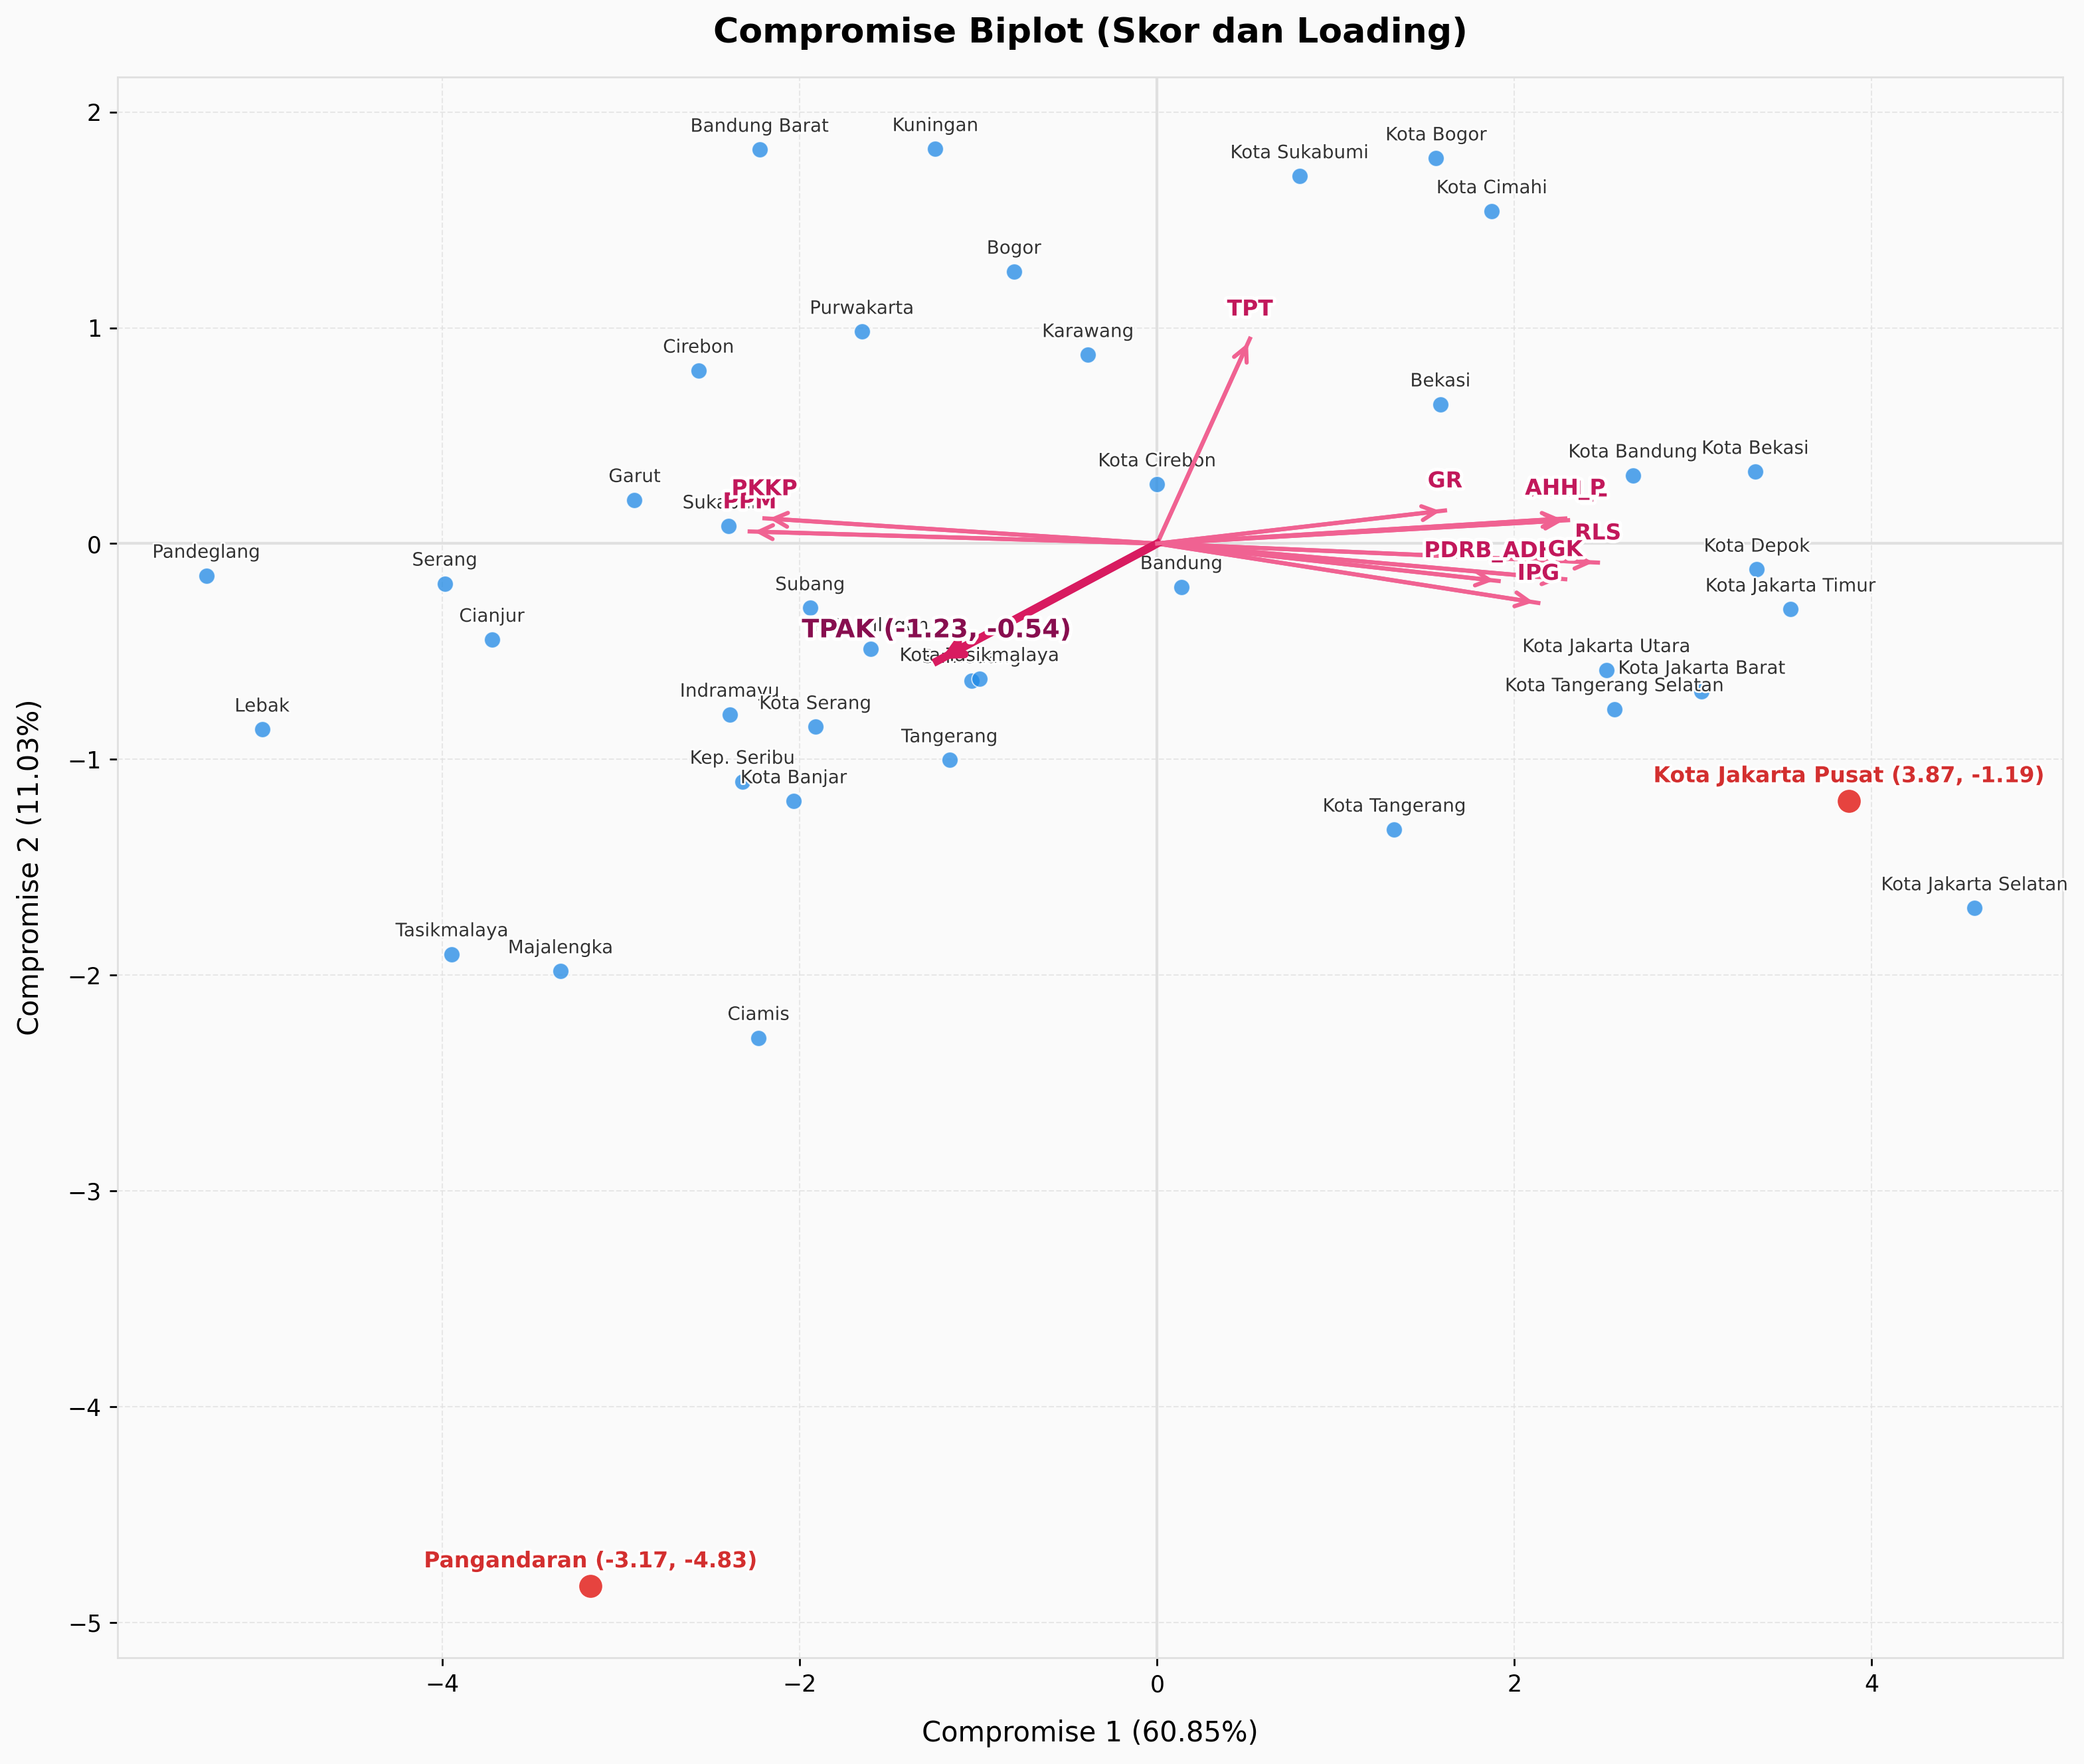
\includegraphics[width=0.75\textwidth]{output_real/scenario1/compromise_biplot.png}
    \caption{Biplot Kompromi Lintas Tahun: Hubungan Struktural antar Wilayah, antar Indikator, dan antar Wilayah dan Indikator}
    \label{fig:biplot_ext_id}
\end{figure}

Pengelompokan lanjut menggunakan algoritma K-Means ($k=3$) pada koordinat kompromi berhasil mempartisi 41 wilayah menjadi tiga kelompok: Klaster~1 ``Tertinggal'' (12 wilayah, didominasi Banten Selatan dan Jawa Barat pedalaman selatan), Klaster~2 ``Berkembang'' (16 wilayah, koridor industri dan penyangga), serta Klaster~3 ``Maju'' (13 wilayah metropolitan). Matriks transisi temporal mengonfirmasi stabilitas sempurna pada 2020--2021, diikuti restrukturisasi terbesar pada 2023--2024 dengan 14 wilayah berpindah dari Klaster~2 ke Klaster~1 dan 4 wilayah dari Klaster~3 ke Klaster~2, sementara sepuluh wilayah metropolitan inti tetap bertahan di Klaster~3 sepanjang seluruh periode. Validasi eksternal terhadap kategori normatif IPM UNDP mengonfirmasi keselarasan struktural yang tinggi, di mana 11 dari 13 anggota Klaster~3 berkategori IPM ``Sangat Tinggi''. Temuan ini mengindikasikan bahwa kesenjangan regional di kawasan Banten--DKI Jakarta--Jawa Barat didorong oleh faktor struktural yang mendalam, sehingga memerlukan intervensi kebijakan yang terarah pada wilayah yang tertinggal, bukan strategi pembangunan yang seragam. Gambar~\ref{fig:traj_ext_id} memperlihatkan pergeseran kondisi sosial ekonomi kabupaten/kota dari tahun ke tahun (2020--2024) yang mencerminkan perbedaan trajektori antar ketiga kelompok tersebut.

\begin{figure}[H]
    \centering
    \captionsetup{hypcap=false}
    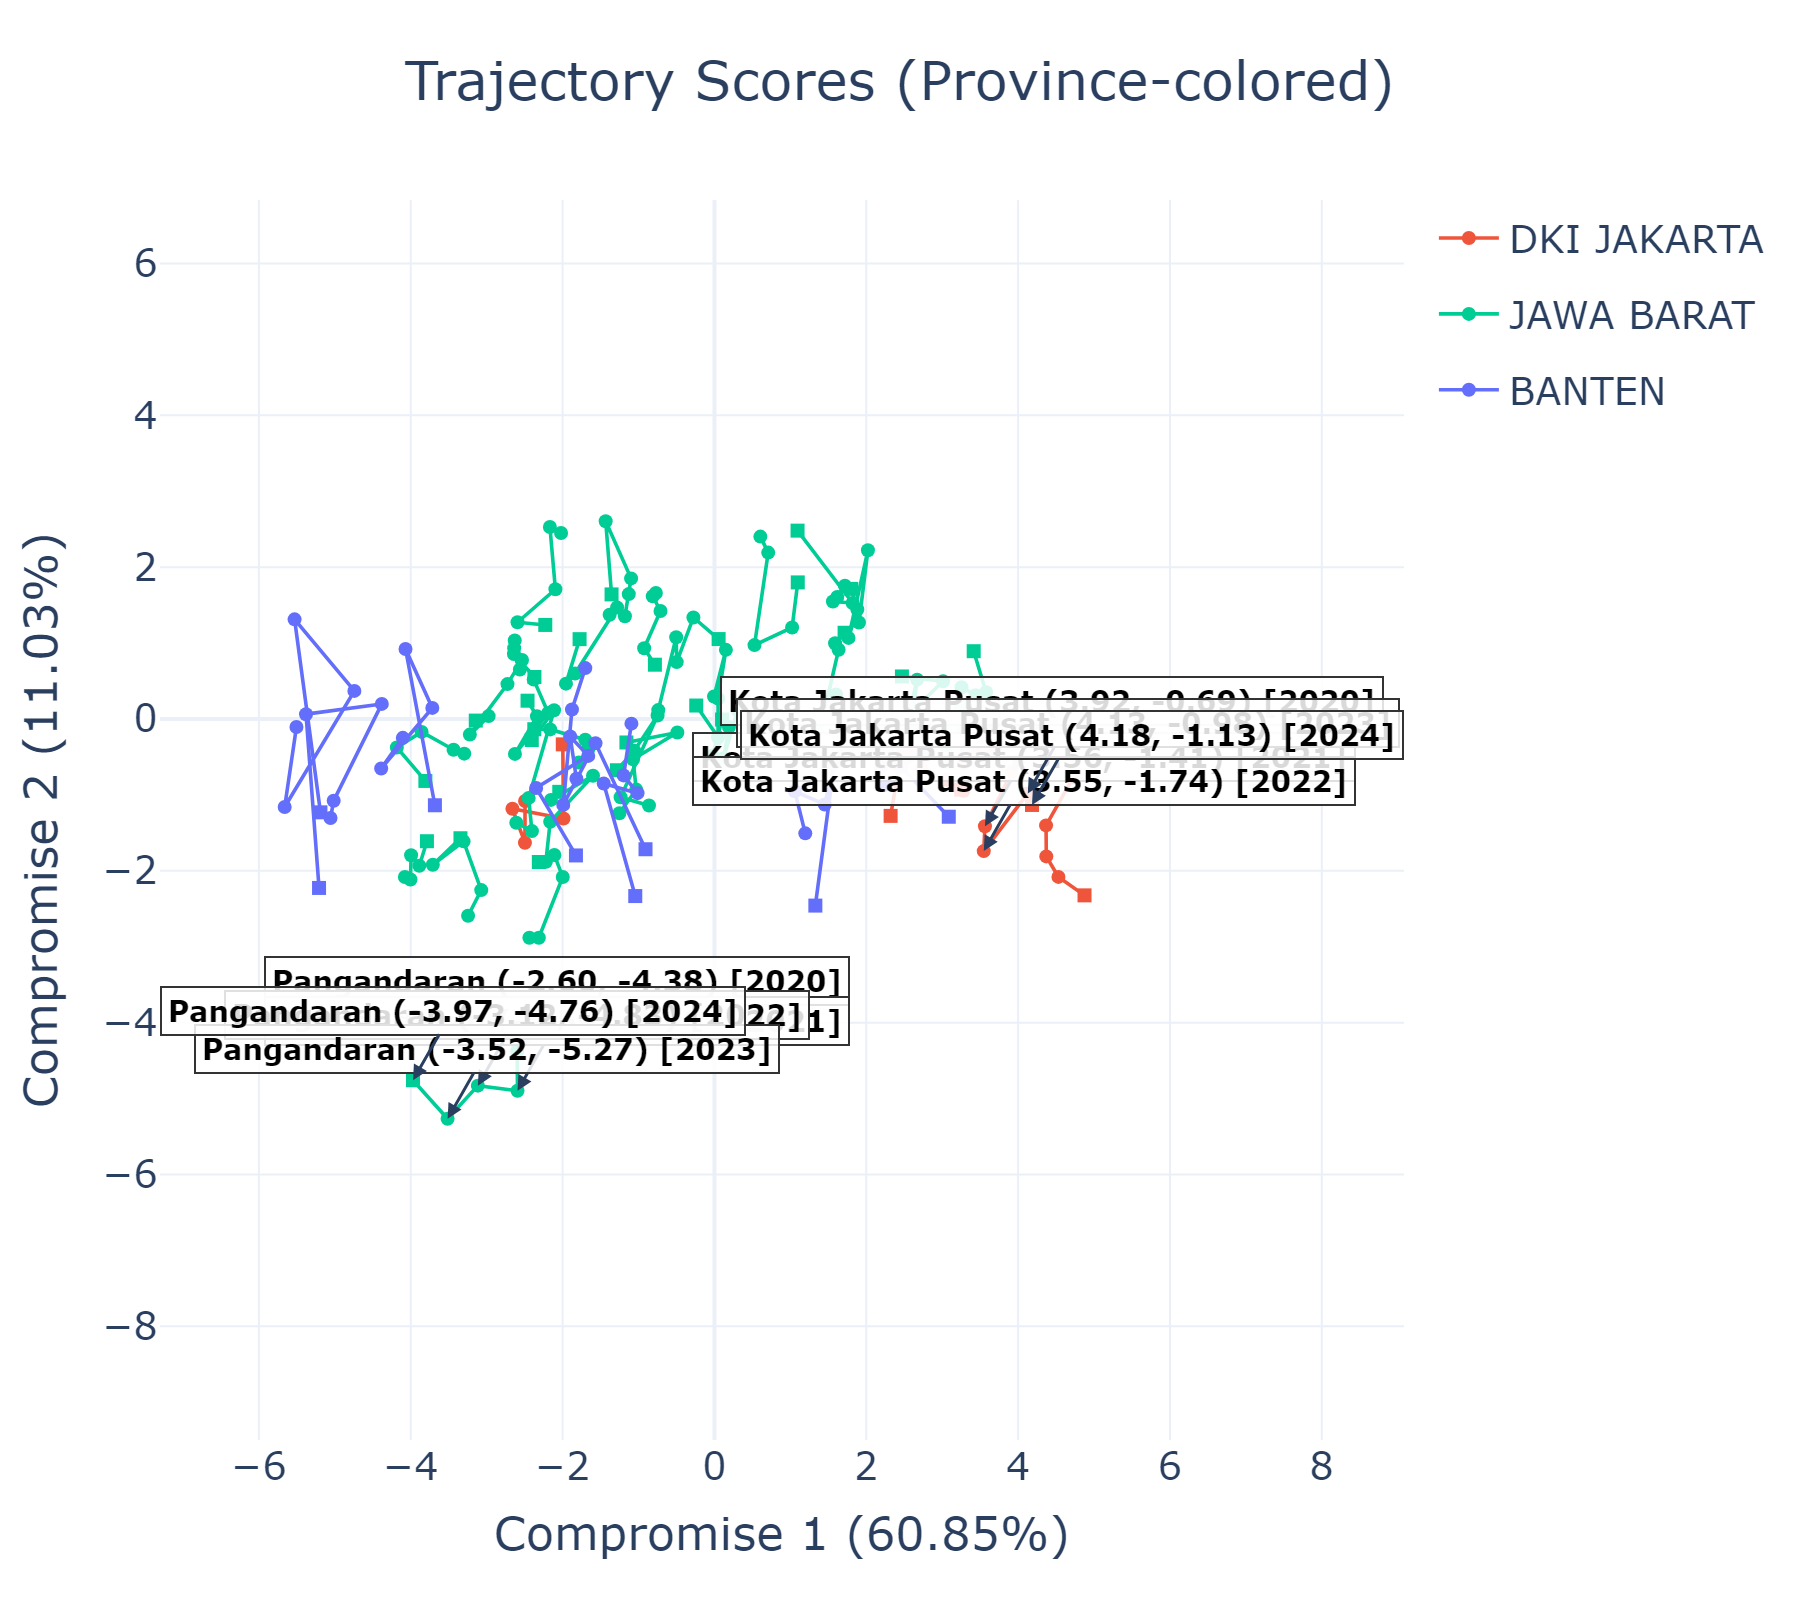
\includegraphics[width=0.75\textwidth]{output_real/scenario1/trajectory_scores.png}
    \caption{Trajektori Spasio-temporal: Pergeseran Kondisi Sosial Ekonomi Kabupaten/Kota dari Tahun ke Tahun (2020--2024)}
    \label{fig:traj_ext_id}
\end{figure}

Sebagai kesimpulan, metode STATIS memberikan perspektif longitudinal yang komprehensif dan melampaui pendekatan analisis statis tradisional dalam memantau dinamika regional. Stabilitas struktural dari representasi kompromi membuktikan bahwa penggerak utama ketimpangan regional bersifat persisten meskipun terjadi pandemi global. Uji permutasi Monte Carlo ($B = 1000$) memvalidasi bahwa struktur yang ditemukan signifikan secara statistik ($p < 0{,}05$) dan bukan merupakan hasil fluktuasi acak. Aplikasi \textit{dashboard} interaktif yang dikembangkan menggunakan \textit{framework} Dash/Plotly menyediakan sarana eksplorasi visual dinamis bagi peneliti dan pemangku kebijakan untuk memantau trajektori pembangunan wilayah secara mandiri dan berbasis data.

\vspace*{0.4cm}

\noindent \bo{Kata Kunci}:
    Analisis Data Tiga Arah, Data Longitudinal, \textit{K-Means Clustering}, PCA, Visualisasi Interaktif.
\vfill
\end{singlespace}

\newpage 
